\documentclass{chapter}

    \author{Xu Jinwen}
    \date{}

    \begin{document}
        \chapter{Complex Analysis, part 1 -  Basic Topics}
        
        \begin{summary}
            This is the first part of book \cite{Stein2003}. In this part we can get familiar with basic notions, methods and ideas in complex analysis.
        \end{summary}

        \section{Introduction, the holomorphicity}\label{section: introduction, holomorphic}
            In this section, we introduce the concept of complex differentiation, \emph{holomorphic}, and show its relationship with real differentiation.

            \bigskip
            The main concern of this subject is what we called \textbf{holomorphic}\index{holomorphic} functions. Roughly speaking, this means the limit \[\frac{f\left(z_{0}+h\right)-f\left(z_{0}\right)}{h}\] exists as $h\to 0$. Here the main difference between the real case is that we allow $h\in\mathbb{C}$. 
            
            \begin{definition}\page{9}
                Let $\Omega$ be an open set in $\mathbb{C}$ and $f$ a complex-valued function on $\Omega$. The function $f$ is holomorphic at the point $z_0 \in \Omega$ if the quotient \[\frac{f\left(z_{0}+h\right)-f\left(z_{0}\right)}{h}\] converges to a limit when $h\to 0$. Here $h\in\mathbb{C}$ and $h\neq 0$ with $z_0 + h \in \Omega$, so that the quotient is well defined.
            \end{definition}
            \begin{remark}
                It should be emphasized that in the above limit, $h$ is a complex number that may approach $0$ from any direction.
            \end{remark}
            
            At first sight this is not a very big difference, but soon we shall see that holomorphic functions has amazing properties.

            \begin{example}
                The function $f(z) = \bar z$ is not holomorphic. Actually, $\frac{f\left(z_{0}+h\right)-f\left(z_{0}\right)}{h}=\frac{\overline{h}}{h}$ has no limit as $h\to 0$, as one can see by first taking $h$ real and then $h$ purely imaginary.

                This example shows that the notion of complex differentiability\index{complex differentiability} differs significantly from the usual notion of real differentiability of a function of two real variables.
            \end{example}

            \bigskip
            First let's take a glance at three most miraculous facts:

            \begin{enumerate}
                \item \textsc{Contour integration}: If $f$ is holomorphic in $\Omega$, then for appropriate closed paths in $\Omega$ \[\int_{\gamma} f(z) \dif z=0.\]
                \item \textsc{Regularity}: If $f$ is holomorphic, then $f$ is indefinitely differentiable.
                \item \textsc{Analytic continuation}: If $f$ and $g$ are holomorphic functions in $\Omega$ which are equal in an arbitrarily small disc in $\Omega$, then $f = g$ everywhere in $\Omega$.
            \end{enumerate}
            
            However, complex differentiation\index{complex differentiation} do have some connections with real differentiability. Indeed, we have the \textbf{Cauchy-Riemann} equations\index{Cauchy-Riemann equations}, which link real and complex analysis. 
        
            Say if we write $h=h_{1}+i h_{2}$, then we have \[\begin{aligned} f^{\prime}\left(z_{0}\right) &=\lim _{h_{1} \rightarrow 0} \frac{f\left(x_{0}+h_{1}, y_{0}\right)-f\left(x_{0}, y_{0}\right)}{h_{1}} \\ &=\frac{\partial f}{\partial x}\left(z_{0}\right). \end{aligned}\] 
            But we also have \[\begin{aligned} f^{\prime}\left(z_{0}\right) &=\lim _{h_{2} \rightarrow 0} \frac{f\left(x_{0}, y_{0}+h_{2}\right)-f\left(x_{0}, y_{0}\right)}{i h_{2}} \\ &=\frac{1}{i} \frac{\partial f}{\partial y}\left(z_{0}\right). \end{aligned}\]
            Thus, \[\frac{\partial f}{\partial x}=\frac{1}{i} \frac{\partial f}{\partial y},\]
            Writing $f = u + iv$, we find after separating real and imaginary parts and using $1/i = -i$, that the partials of $u$ and $v$ exist, and they satisfy the following non-trivial relations.
            
            \begin{theorem}[the Cauchy-Riemann equations]\page{12}
                \[\frac{\partial u}{\partial x}=\frac{\partial v}{\partial y} \quad \text { and } \quad \frac{\partial u}{\partial y}=-\frac{\partial v}{\partial x}.\]
            \end{theorem}

            \bigskip
            If we define two differential operators\index{differential operator} \[\frac{\partial}{\partial z}=\frac{1}{2}\left(\frac{\partial}{\partial x}+\frac{1}{i} \frac{\partial}{\partial y}\right) \quad \text { and } \quad \frac{\partial}{\partial \overline{z}}=\frac{1}{2}\left(\frac{\partial}{\partial x}-\frac{1}{i} \frac{\partial}{\partial y}\right)\page{12}\]\index{$\frac{\partial}{\partial z}$}\index{$\frac{\partial}{\partial \overline{z}}$} 
            \begin{remark}
                The definition of $\frac{\partial}{\partial z}$ and $\frac{\partial}{\partial \overline{z}}$ is motivated by noticing that $x=\frac{z+\overline z}{2}$, $y=\frac{z-\overline z}{2i}$ and then using the chain rule. We can therefore get $\frac{\partial f}{\partial z}=\frac{1}{2}\left(\frac{\partial f}{\partial x}+\frac{1}{i} \frac{\partial f}{\partial y}\right)$ and $\frac{\partial f}{\partial \overline{z}}=\frac{1}{2}\left(\frac{\partial f}{\partial x}-\frac{1}{i} \frac{\partial f}{\partial y}\right)$.
            \end{remark}

            Then we have

            \begin{theorem}[from complex differentiation to real differentiability]\page{12}
                If $f$ is holomorphic at $z_0$, then \[\frac{\partial f}{\partial \overline{z}}\left(z_{0}\right)=0 \quad \text { and } \quad f^{\prime}\left(z_{0}\right)=\frac{\partial f}{\partial z}\left(z_{0}\right)=2 \frac{\partial u}{\partial z}\left(z_{0}\right).\]
                Also, if we write $F(x, y) = f(z)$, then $F$ is differentiable in the sense of real variables, and \[\operatorname{det} J_{F}\left(x_{0}, y_{0}\right)=\left|f^{\prime}\left(z_{0}\right)\right|^{2}.\]
            \end{theorem}

            The next theorem contains an important converse, which completes the circle of ideas presented here.
            
            \begin{theorem}[from real differentiation to complex differentiability]\page{13}
                Suppose $f = u + iv$ is a complex-valued function defined on an open set $\Omega$. If $u$ and $v$ are continuously differentiable and satisfy the Cauchy-Riemann equations on $\Omega$, then $f$ is holomorphic on $\Omega$ and $f^{\prime}(z)=\partial f / \partial z$.
            \end{theorem}

        \section{Power series and analytic}\label{section: power series and analytic}
            In this section we discuss some basic properties of power series, which will be useful in later studies.

            \bigskip
            In general, a \textbf{power series}\index{power series} centered at $z_{0}$ is an expansion of the form \[f(z)=\sum_{n=0}^{\infty} a_{n}\left(z-z_{0}\right)^{n}\] where $a_n\in\mathbb{C}$. By making some translation, we can simply deal with power series centered at the origin \[\sum_{n=0}^{\infty} a_{n} z^{n}.\] 
            
            An important fact is that there always exists an open disc (possibly empty) on which the power series converges absolutely.

            \begin{theorem}\page{15}
                Given a power series $\sum_{n=0}^{\infty} a_{n} z^{n}$, there exists $0 \leq R \leq \infty$ such that:

                \begin{enumerate}
                    \item If $|z|<R$ the series converges absolutely.
                    \item If $|z|>R$ the series diverges.
                \end{enumerate}

                Moreover, if we use the convention that $1 / 0=\infty$ and $1 / \infty=0,$ then $R$ is given by Hadamard's formula \[1 / R=\limsup \left|a_{n}\right|^{1 / n}.\]
            \end{theorem}

            The number $R$ is called the \textbf{radius of convergence}\index{radius of convergence} of the power series, and the region $|z|<R$ the \textbf{disc of convergence}\index{disc of convergence}.

            \begin{remark}
                On the boundary of the disc of convergence, $|z|=R,$ the situation is more delicate as one can have either convergence or divergence.
            \end{remark}

            \begin{example}
                The prime example of a power series is the complex exponential function, which is defined for $z \in \mathbb{C}$ by \[e^{z}=\sum_{n=0}^{\infty} \frac{z^{n}}{n !}\]
                When $z$ is real, this definition coincides with the usual exponential function, and in fact, the series above converges absolutely for every $z \in \mathbb{C}$.
            \end{example}

            \begin{example}
                In contrast, the geometric series \[\sum_{n=0}^{\infty} z^{n}\] converges absolutely only in the disc $|z|<1,$ and its sum there is the function $1 /(1-z),$ which is holomorphic in the open set $\mathbb{C}-\{1\}.$ 
            \end{example}

            \begin{example}
                Further examples of power series that converge in the whole complex plane are given by the standard \textbf{trigonometric functions}\index{trigonometric functions}; these are defined by \[\cos z=\sum_{n=0}^{\infty}(-1)^{n} \frac{z^{2 n}}{(2 n) !}, \quad \text { and } \quad \sin z=\sum_{n=0}^{\infty}(-1)^{n} \frac{z^{2 n+1}}{(2 n+1) !}\] and they agree with the usual cosine and sine of a real argument whenever $z \in \mathbb{R} .$ A simple calculation exhibits a connection between these two functions and the complex exponential, namely, \[\cos z=\frac{e^{i z}+e^{-i z}}{2} \quad \text { and } \quad \sin z=\frac{e^{i z}-e^{-i z}}{2 i}.\] These are called the \textbf{Euler formulas}\index{Euler formulas} for the cosine and sine functions.
            \end{example}

            \bigskip
            Power series provide a very important class of analytic functions that are particularly simple to manipulate. For example, we have

            \begin{theorem}[analytic to holomorphic, differentiation by term of power series]\page{16}
                The power series $f(z)=\sum_{n=0}^{\infty} a_{n} z^{n}$ defines a holomorphic function in its disc of convergence. The derivative of $f$ is also a power series obtained by differentiating term by term the series for $f$, that is, \[f^{\prime}(z)=\sum_{n=0}^{\infty} n a_{n} z^{n-1}.\] Moreover, $f^{\prime}$ has the same radius of convergence as $f$.
                \label{theorem: analytic to holomorphic}
            \end{theorem}
            \begin{corollary}
                A power series is infinitely complex differentiable in its disc of convergence, and the higher derivatives are also power series obtained by termwise differentiation.
            \end{corollary}

            \begin{definition}[analytic]\page{18}
                A function $f$ defined on an open set $\Omega$ is said to be \textbf{analytic}\index{analytic} (or have a \textbf{power series expansion}\index{power series!expansion}) at a point $z_{0} \in \Omega$ if there exists a power series $\sum a_{n}\left(z-z_{0}\right)^{n}$ centered at $z_{0}$, with positive radius of convergence, such that \[f(z)=\sum_{n=0}^{\infty} a_{n}\left(z-z_{0}\right)^{n} \quad \text { for all } z \text { in a neighborhood of } z_{0}.\]

                If $f$ has a power series expansion at every point in $\Omega$, we say that $f$ is \textbf{analytic on $\Omega$}.
            \end{definition}
            
            \bigskip
            Theorem \ref{theorem: analytic to holomorphic} shows that an analytic function on $\Omega$ is also holomorphic there. A deep theorem which we prove later (Theorem \ref{theorem: holomorphic to analytic}) says that the converse is true: every holomorphic function is analytic. For that reason, we use the terms holomorphic and analytic interchangeably.

            \begin{remark}
                Notice that this is obviously not true for the real case. Thus we can see that holomorphic is a very strong condition.
            \end{remark}

            \bigskip
            Surprisingly enough, to study the properties of complex differentiation further, we will need the tools of integration. Thus let's return to this topic later and look at the complex integration for now.

        \section{Complex integration and integration along curves}

            \begin{definition}[integration along curves]\page{21}\index{integration!along curves}
                Given a smooth curve $\gamma$ in $\mathbb{C}$ parametrized by $z :[a, b] \to \mathbb{C}$, and $f$ a continuous function on $\gamma$, we define the \textbf{integral of $f$ along $\gamma$} by \[\int_{\gamma} f(z) \dif z=\int_{a}^{b} f(z(t)) z^{\prime}(t) \dif t.\]
            \end{definition}

            \begin{remark}
                Notice that the change of variables formula and the chain rule, \[\int_{a}^{b} f(z(t)) z^{\prime}(t) \dif t=\int_{c}^{d} f(z(t(s))) z^{\prime}(t(s)) t^{\prime}(s) \dif s=\int_{c}^{d} f(\tilde{z}(s)) \tilde{z}^{\prime}(s) \dif s,\] which proves that the integral of $f$ over $\gamma$ is well defined.
            \end{remark}

            \begin{proposition}\page{21}
                Integration of continuous functions over curves satisfies the following properties:
                \begin{enumerate}
                    \item It is linear, that is, if $\alpha, \beta \in \mathbb{C},$ then \[\int_{\gamma}(\alpha f(z)+\beta g(z)) \dif z=\alpha \int_{\gamma} f(z) \dif z+\beta \int_{\gamma} g(z) \dif z.\]
                    \item If $\gamma^{-}$ is $\gamma$ with the reverse orientation, then \[\int_{\gamma} f(z) \dif z=-\int_{\gamma^{-}} f(z) \dif z.\]
                    \item One has the inequality \[\left|\int_{\gamma} f(z) \dif z\right| \leq \sup _{z \in \gamma}|f(z)| \cdot \operatorname{length}(\gamma).\] Here, the length of the smooth curve $\gamma$ is \[\operatorname{length}(\gamma)=\int_{a}^{b}\left|z^{\prime}(t)\right| \dif t.\]
                \end{enumerate}
            \end{proposition}

            \bigskip
            As introduced in section \ref{section: introduction, holomorphic}, Cauchy's theorem states that for appropriate closed curves $\gamma$ in an open set $\Omega$ on which $f$ is holomorphic, then \[\int_{\gamma} f(z) \dif z=0.\] The existence of primitives gives a first manifestation of this phenomenon.

            \begin{definition}[primitive]\page{22}
                Suppose $f$ is a function on the open set $\Omega .$ A \textbf{primitive}\index{primitive} for $f$ on $\Omega$ is a function $F$ that is holomorphic on $\Omega$ and such that $F^{\prime}(z)=f(z)$ for all $z \in \Omega$.
            \end{definition}

            The existence of primitive gives us a sense of \emph{path independence}.

            \begin{theorem}\page{22}
                If a continuous function $f$ has a primitive $F$ in $\Omega,$ and $\gamma$ is a curve in $\Omega$ that begins at $w_{1}$ and ends at $w_{2},$ then \[\int_{\gamma} f(z) \dif z=F\left(w_{2}\right)-F\left(w_{1}\right).\]
            \end{theorem}

            Since the end-points of a closed curve coincide, we have:

            \begin{corollary}
                If $\gamma$ is a closed curve in an open set $\Omega,$ and $f$ is continuous and has a primitive in $\Omega,$ then \[\int_{\gamma} f(z) \dif z=0.\]
            \end{corollary}

            \begin{example}
                For example, the function $f(z)=1 / z$ does not have a primitive in the open set $\mathbb{C}-\{0\},$ since if $C$ is the unit circle parametrized by $z(t)=e^{i t}$, $0 \leq t \leq 2 \pi,$ we have \[\int_{C} f(z) \dif z=\int_{0}^{2 \pi} \frac{i e^{i t}}{e^{i t}} \dif t=2 \pi i \neq 0.\]
            \end{example}

            As will be discussed in the next section, this innocent calculation, which provides an example of a function $f$ and closed curve $\gamma$ for which $\int_{\gamma} f(z) \dif z \neq 0$, lies at the heart of the theory.

        \section{Cauchy’s theorem}
            We take Goursat's way to the Cauchy's theorem. Our starting point is Goursat’s theorem, from which in effect we shall deduce most of the other results in this section.

            \begin{theorem}[Goursat’s theorem]\page{34}
                If $\Omega$ is an open set in $\mathbb{C},$ and $T \subset \Omega$ a triangle whose interior is also contained in $\Omega,$ then \[\int_{T} f(z) \dif z=0\] whenever $f$ is holomorphic in $\Omega$.
            \end{theorem}

            \begin{remark}
                The technique of its proof is important and deserve your attention. It's basic idea is shown in the picture below.

                \begin{center}
                    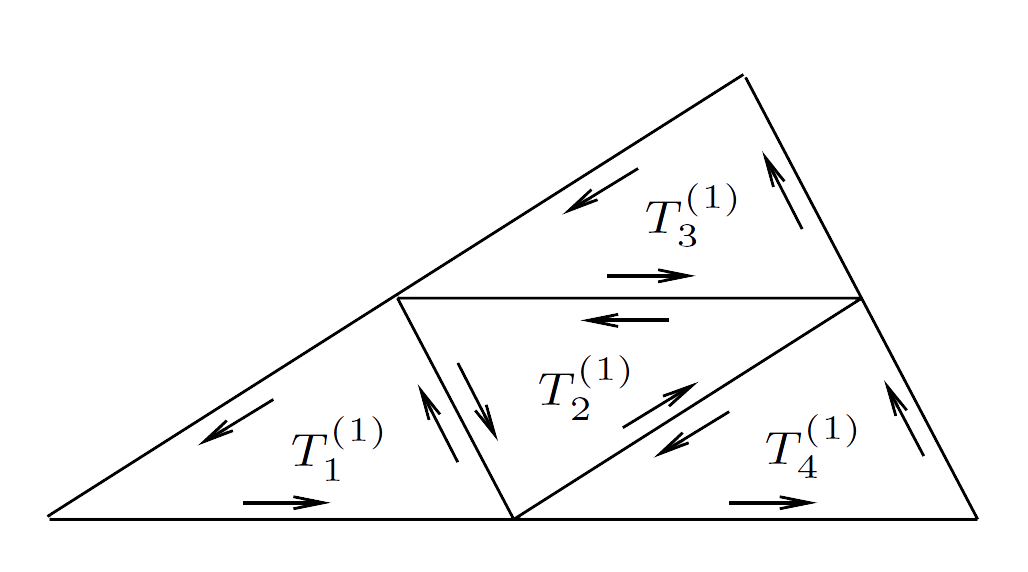
\includegraphics[width=5cm]{ComplexAnalysis/ch2-Bisection_of_T.png}
                \end{center}
            \end{remark}
            
            Using this result for triangle we can prove for some more general settings such as discs, and in this book, toy contours. The basic ideas and an example of toy contours are shown below.

            \begin{center}
                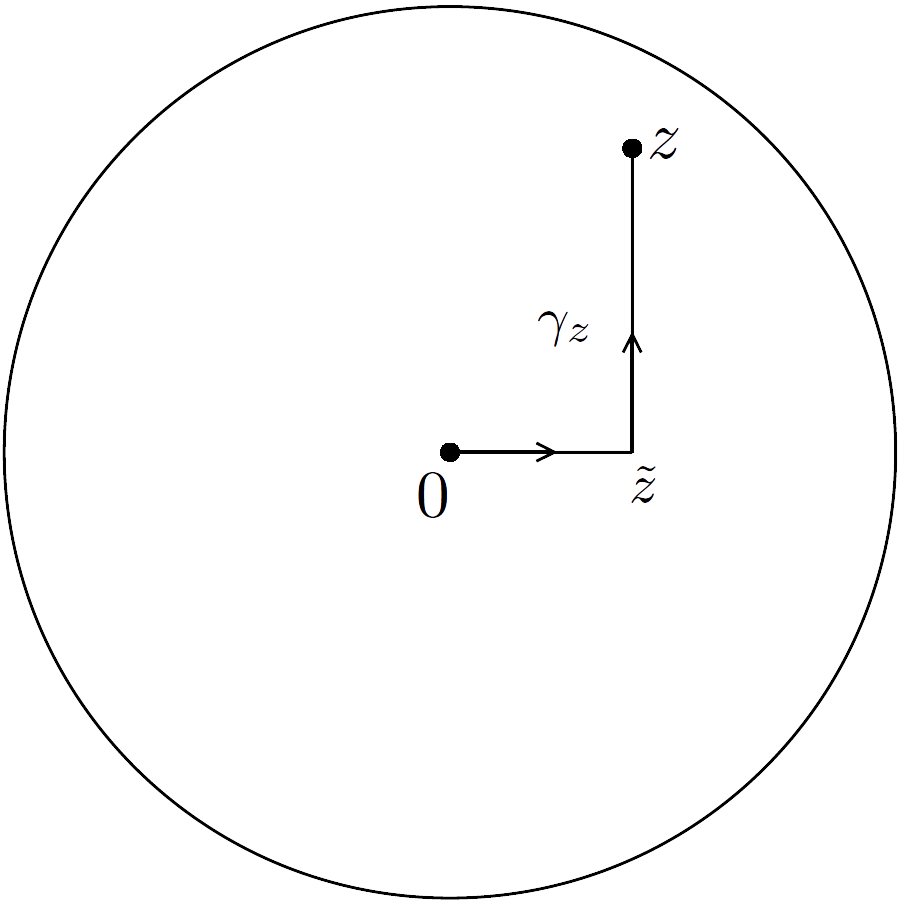
\includegraphics[height=4cm]{ComplexAnalysis/ch2-the_polygonal_line.png}
                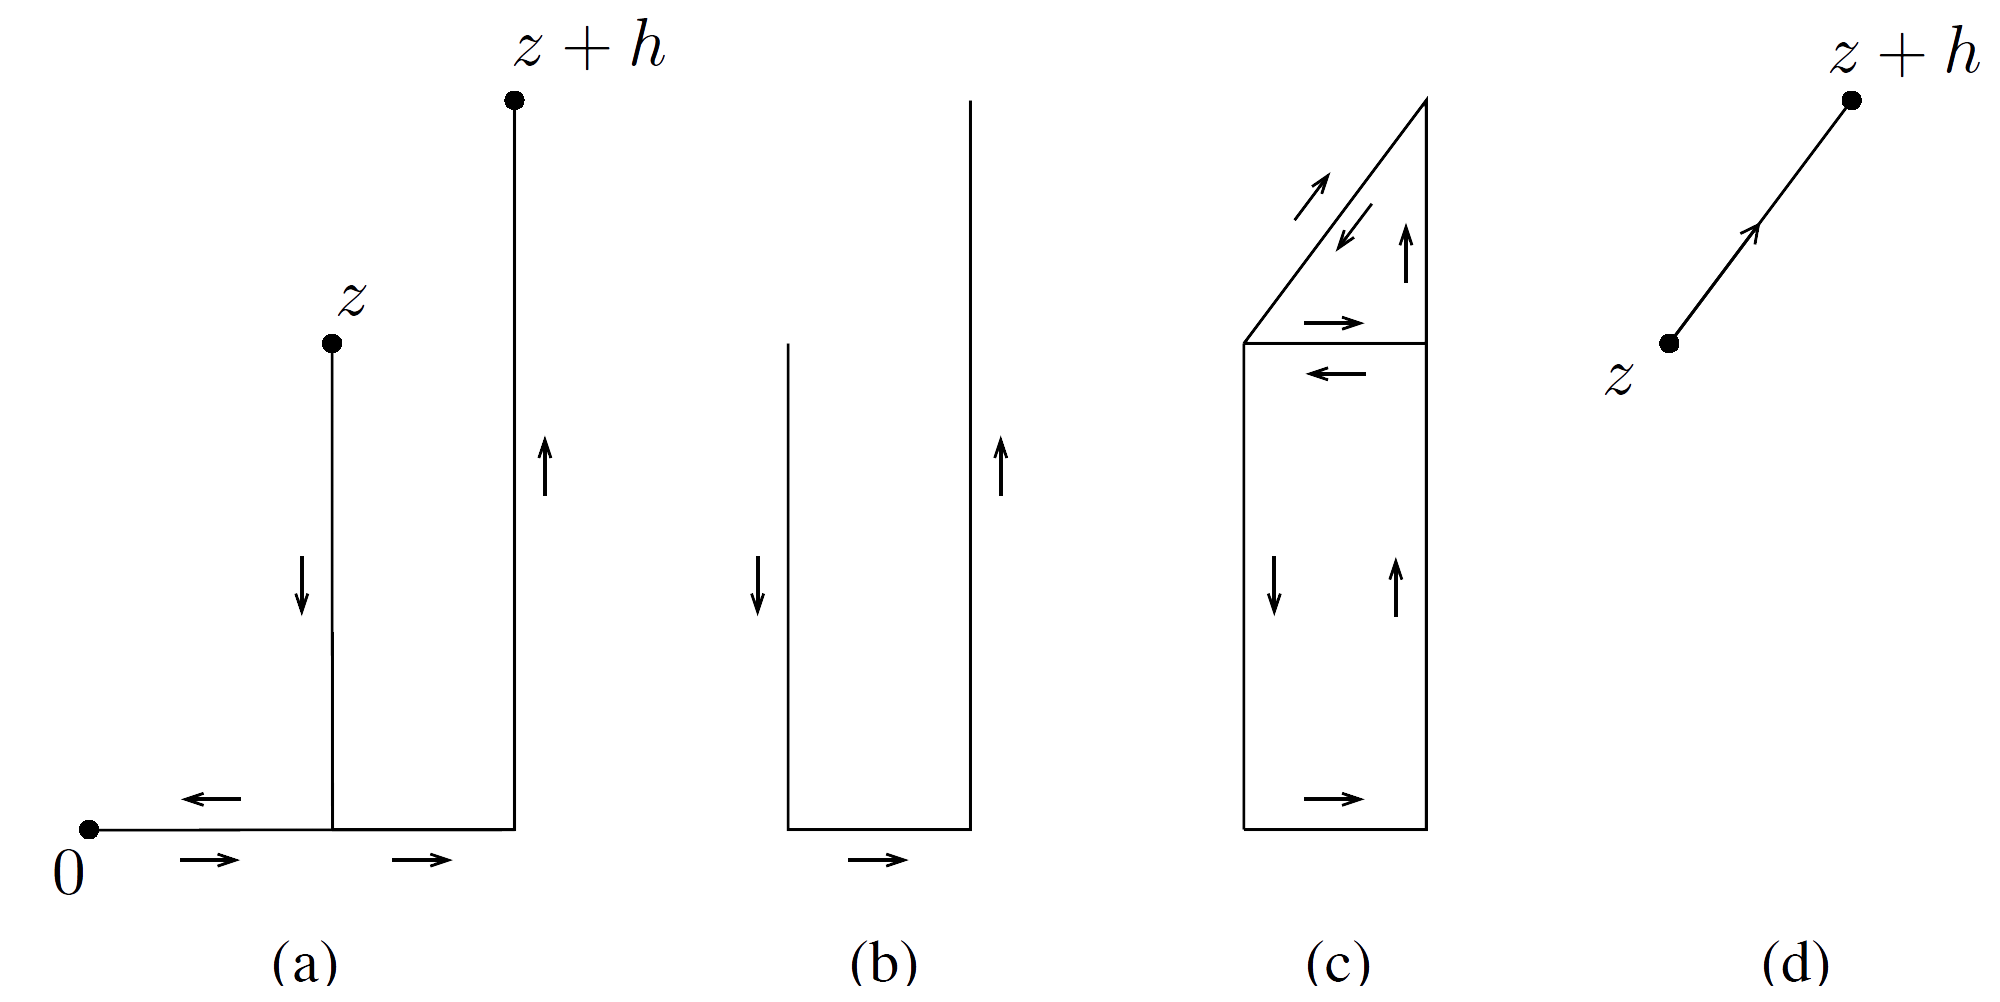
\includegraphics[height=4cm]{ComplexAnalysis/ch2-Relation_between_the_polygonal_lines.png}
                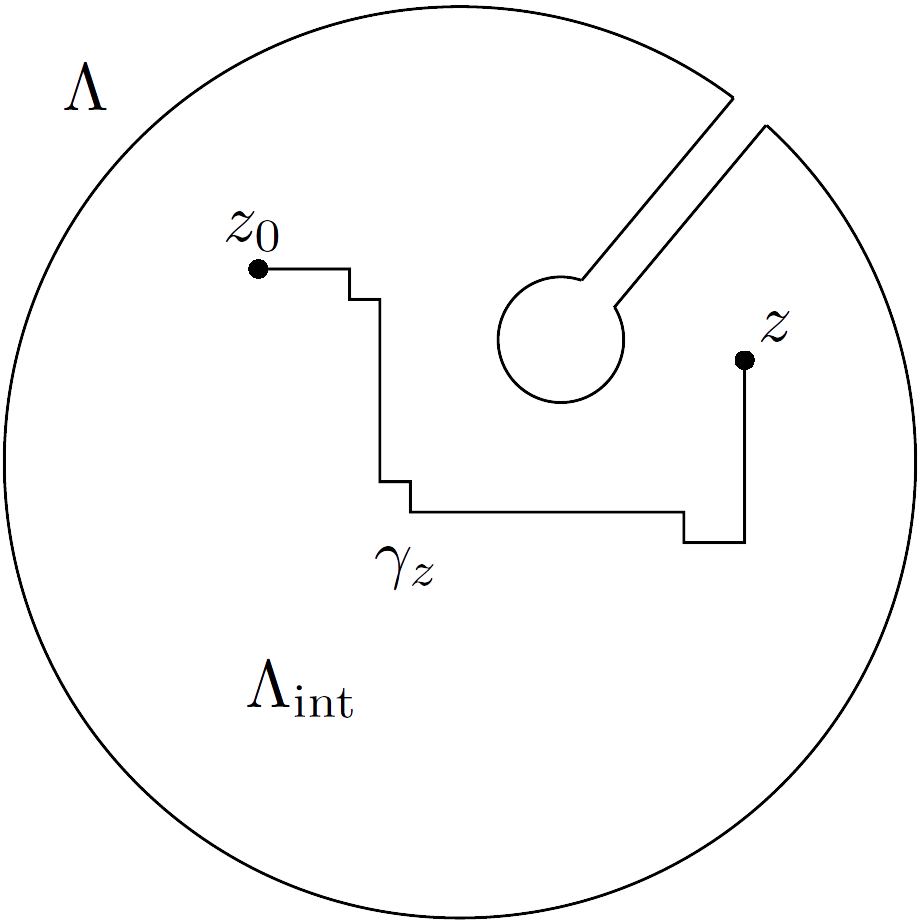
\includegraphics[height=4cm]{ComplexAnalysis/ch2-The_keyhole_contour.png}
            \end{center}

            Using the idea illustrated above, we can prove that for certain cases the primitive does exist.

            \begin{theorem}\page{37}
                A holomorphic function in an open disc has a primitive in that disc.
                \label{theorem: exist primitive}
            \end{theorem}

            \begin{remark}
                It would be enough using discs as examples to illustrate the main idea, and therefore, though many results concerns only discs, their idea can be taken to many other much complicated cases.
            \end{remark}

            The general version of the Cauchy’s theorem can be stated as
            \begin{theorem}[Cauchy’s theorem]\page{352}
                Suppose $f$ is a function that is holomorphic in the interior $\Omega$ of a simple closed curve $\Gamma$. Then \[\int_{\eta} f(\zeta) \dif \zeta=0\] whenever $\eta$ is any closed curve contained in $\Omega$.
            \end{theorem}

            \bigskip
            We can use this theorem to calculate some sophisticated integrals.

            \begin{example}
                We show that if $\xi \in \mathbb{R},$ then \[e^{-\pi \xi^{2}}=\int_{-\infty}^{\infty} e^{-\pi x^{2}} e^{-2 \pi i x \xi} \dif x.\]
            \end{example}

            \begin{example}
                Another classical example is \[\int_{0}^{\infty} \frac{1-\cos x}{x^{2}} \dif x=\frac{\pi}{2}.\]
            \end{example}

            Representation formulas, and in particular integral representation formulas, play an important role in mathematics, since they allow us to recover a function on a large set from its behavior on a smaller set. This is particularly the case when we are dealing with elliptic functions. As for now, we have the following Cauchy’s integral formula\index{Cauchy’s integral formula}.

            \begin{theorem}[Cauchy’s integral formula I]\page{45}
                Suppose $f$ is holomorphic in an open set that contains the closure of a disc $D$. If $C$ denotes the boundary circle of this disc with the positive orientation, then \[f(z)=\frac{1}{2 \pi i} \int_{C} \frac{f(\zeta)}{\zeta-z} \dif \zeta \quad \text { for any point } z \in D.\]
            \end{theorem}
            \begin{remark}
                It should be noted that the above integral vanishes when $z$ is outside $R,$ since in this case $F(\zeta)=f(\zeta) /(\zeta-z)$ is holomorphic inside $R$.
            \end{remark}

            We have the following very insightful corollaries.
            \begin{corollary}[Cauchy’s integral formula II]\page{47}
                If $f$ is holomorphic in an open set $\Omega,$ then $f$ has infinitely many complex derivatives in $\Omega$. Moreover, if $C \subset \Omega$ is a circle whose interior is also contained in $\Omega,$ then \[f^{(n)}(z)=\frac{n !}{2 \pi i} \int_{C} \frac{f(\zeta)}{(\zeta-z)^{n+1}} d \zeta\] for all $z$ in the interior of $C$.
            \end{corollary}

            \begin{corollary}[Cauchy inequalities]\page{48}
                If $f$ is holomorphic in an open set that contains the closure of a disc $D$ centered at $z_0$ and of radius $R$, then \[\left|f^{(n)}\left(z_{0}\right)\right| \leq \frac{n !\|f\|_{C}}{R^{n}},\] where $\|f\|_{C}=\sup _{z \in C}|f(z)|$ denotes the supremum of $|f|$ on the boundary circle $C$.
            \end{corollary}

            Another striking consequence of the Cauchy integral formula is its connection with power series. In section \ref{section: power series and analytic}, we proved that a power series is holomorphic in the interior of its disc of convergence, and promised a proof of a converse, which is the content of the next theorem.
            
            \begin{theorem}[holomorphic to analytic]\page{49}
                Suppose $f$ is holomorphic in an open set $\Omega$. If $D$ is a disc centered at $z_{0}$ and whose closure is contained in $\Omega,$ then $f$ has a power series expansion at $z_{0}$ \[f(z)=\sum_{n=0}^{\infty} a_{n}\left(z-z_{0}\right)^{n}\] for all $z \in D$, and the coefficients are given by \[a_{n}=\frac{f^{(n)}\left(z_{0}\right)}{n !} \quad \text { for all } n \geq 0.\]
                \label{theorem: holomorphic to analytic}
            \end{theorem}
            \begin{remark}
                Notice that the main idea in its proof is to write \[\frac{1}{\zeta-z}=\frac{1}{\zeta-z_{0}-\left(z-z_{0}\right)}=\frac{1}{\zeta-z_{0}} \frac{1}{1-\left(\frac{z-z_{0}}{\zeta-z_{0}}\right)},\] and then use \[\frac{1}{1-\left(\frac{z-z_{0}}{\zeta-z_{0}}\right)}=\sum_{n=0}^{\infty}\left(\frac{z-z_{0}}{\zeta-z_{0}}\right)^{n}.\]
            \end{remark}

            In particular, if $f$ is entire (that is, holomorphic on all of $\mathbb{C}$), the theorem implies that $f$ has a power series expansion around $0,$ say $f(z)=\sum_{n=0}^{\infty} a_{n} z^{n},$ that converges in all of $\mathbb{C}$.

            \begin{corollary}[Liouville’s theorem]\page{50}
                If $f$ is entire and bounded, then $f$ is constant.
            \end{corollary}
            \begin{remark}
                The main idea is to show that $f^{\prime}=0$ by using the Cauchy inequalities.
            \end{remark}

            It can be used to prove the fundamental theorem of algebra. How amazing!
            \begin{corollary}[the fundamental theorem of algebra]\page{50}
                Every non-constant polynomial $P(z)=a_{n} z^{n}+\cdots+a_{0}$ with complex coefficients has a root in $\mathbb{C}$.
            \end{corollary}

            \bigskip
            Finally, we end this section with a discussion of analytic continuation (the third of the “miracles” we mentioned in the introduction). It states that the “genetic code” of a holomorphic function is determined (that is, the function is fixed) if we know its values on appropriate arbitrarily small subsets. Note that in the theorem below, $\Omega$ is assumed connected.

            \begin{theorem}\page{52}
                Suppose $f$ is a holomorphic function in a region $\Omega$ that vanishes on a sequence of distinct points with a limit point in $\Omega$. Then $f$ is identically $0$.
            \end{theorem}
            This is the stronger statement. What we are really interested in is the following
            \begin{corollary}[uniqueness of analytic continuation]\page{52}
                Suppose $f$ and $g$ are holomorphic in a region $\Omega$ and $f(z)=g(z)$ for all $z$ in some non-empty open subset of $\Omega$ (or more generally for $z$ in some sequence of distinct points with limit point in $\Omega$). Then $f(z)=g(z)$ throughout $\Omega$.
            \end{corollary}
            Suppose we are given a pair of functions $f$ and $F$ analytic in regions $\Omega$ and $\Omega^{\prime},$ respectively, with $\Omega \subset \Omega^{\prime}$. If the two functions agree on the smaller set $\Omega$, we say that $F$ is an \textbf{analytic continuation}\index{analytic continuation} of $f$ into the region $\Omega^{\prime}$. The corollary then guarantees that there can be only one such analytic continuation, since $F$ is uniquely determined by $f$.

        \section{Further applications of Cauchy's theorem}
            \begin{theorem}[Morera’s theorem]
                Suppose $f$ is a continuous function in the open disc $D$ such that for any triangle $T$ contained in $D$ \[\int_{T} f(z) d z=0\] then $f$ is holomorphic.
            \end{theorem}
            \begin{remark}
                The key observation is that $f$ has a primitive $F$ in $D$ using the idea of Theorem \ref{theorem: exist primitive}.
            \end{remark}
    \end{document}